\lab{Principal Component Analysis}{Principal Component Analysis}
\objective{Understand the basics of principal component analysis}

Understanding the variance in complex data is one of the initial tasks in exploratory data analysis. For example, consider the following scatter plot (Figure \ref{fig:iris_1}) displaying the sepal and petal lengths of 100 different irises.
\begin{figure}
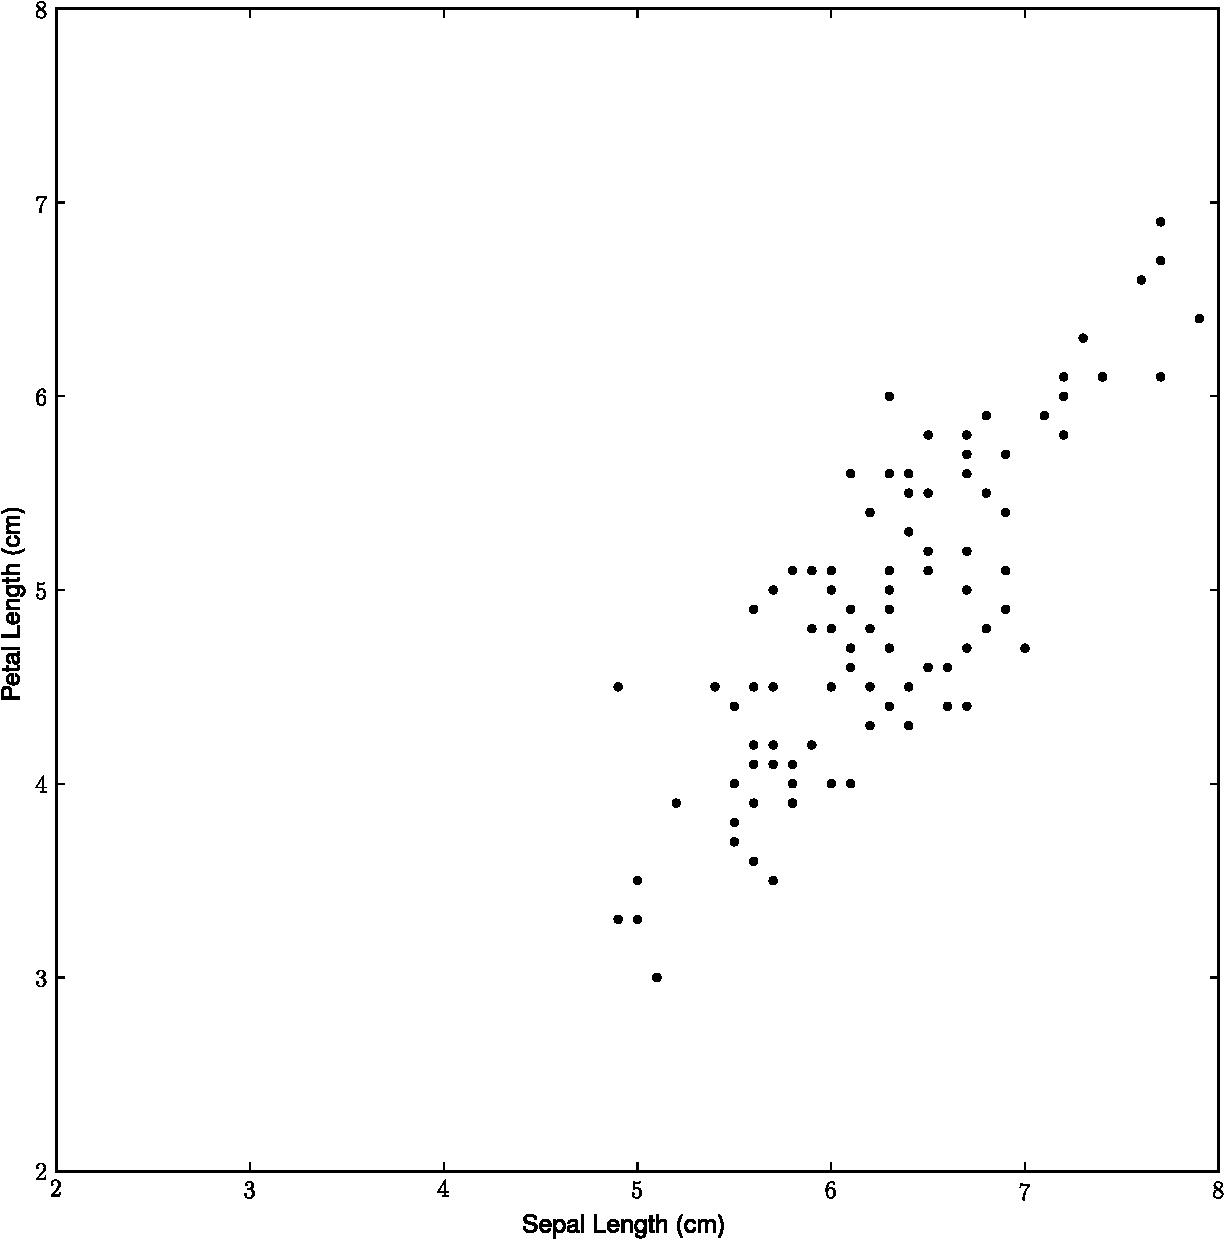
\includegraphics[width=\textwidth]{iris0.pdf}
\caption{Note the strong correlation of these variables.}
\label{fig:iris_1}
\end{figure}
Considering this data, we might ask what aspect of irises is most distinguishing (causes the greatest variance). Upon examination, we might see that the petal length ranges between $3$ and $7$ cm, while the sepal length only ranges between $5$ and $8$. So we might be tempted to say that the most distinguishing aspect of irises is their petal length, but this is only considering the features of the data individually, and not collectively. This data is clearly correlated, and a more careful consideration would lead us to conclude that the most distinguishing aspect of irises is their overall size. Some irises are are much bigger than others while the sepal and petal lengths stay roughly in proportion.
\begin{figure}
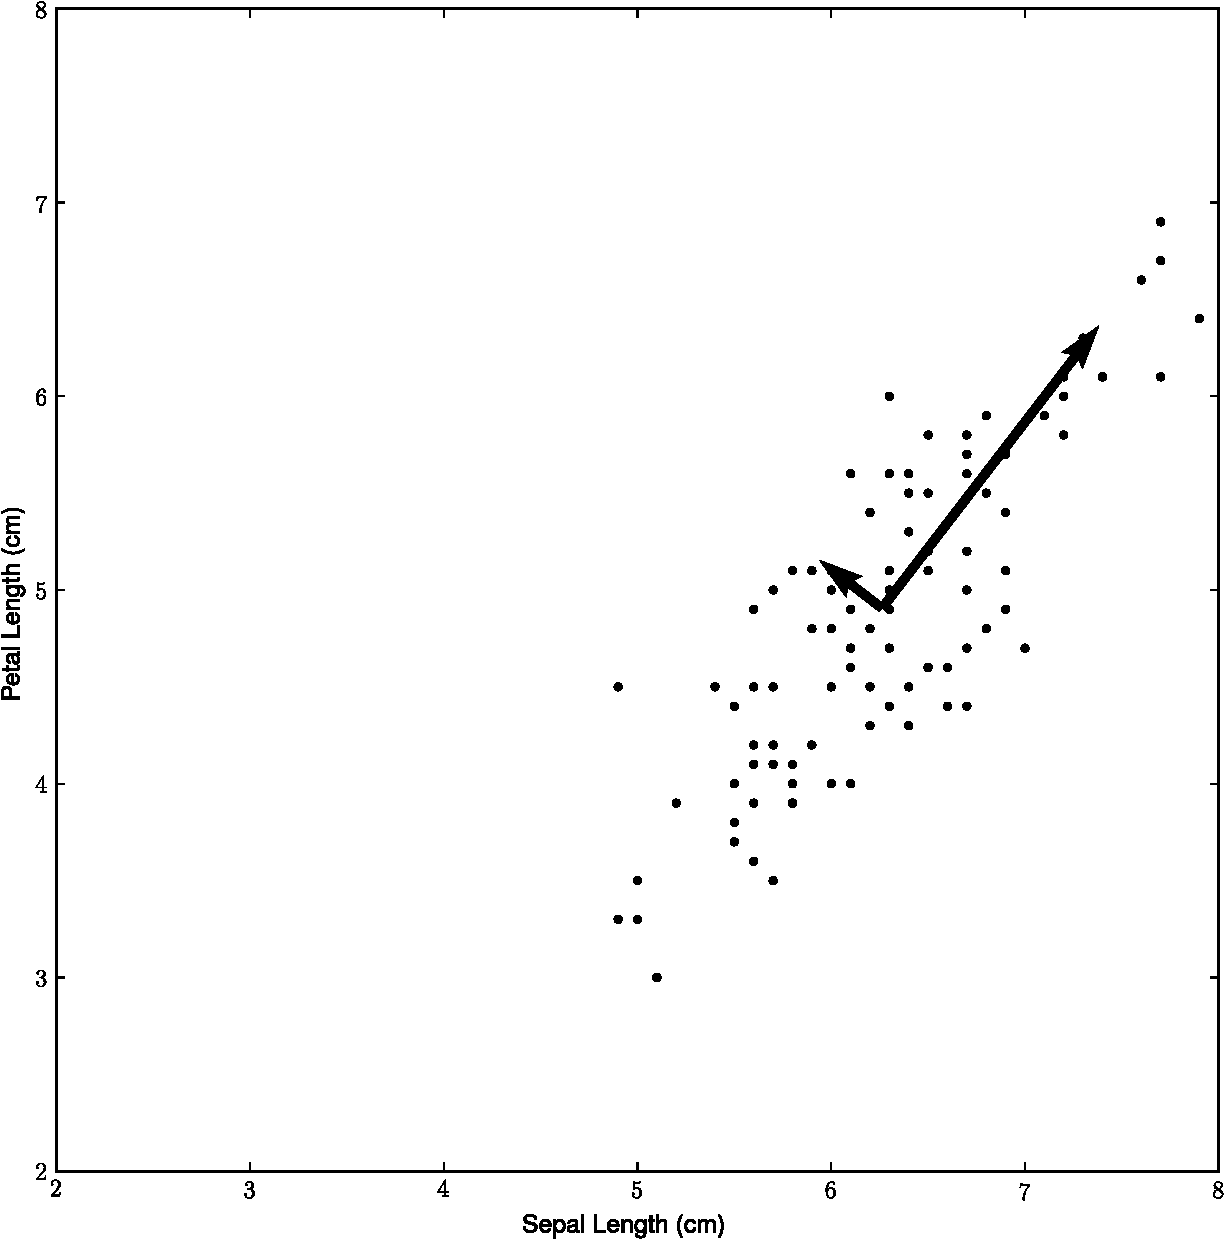
\includegraphics[width=\textwidth]{iris2.pdf}
\caption{The vectors indicate the two principal components.}
\label{fig:iris_2}
\end{figure}

Principal Component Analysis (PCA) is a multivariate statistical tool used to orthogonally transform a set of observations over multiple features which may be correlated into a set of values whose variables are linearly uncorrelated. It is a direct application of the singular value decomposition (SVD) from linear algebra. More specifically, the first new variable will account for the greatest variance in the set of observations, the second variable will be orthogonal to the first, accounting for the second greatest variance in the set of observations, etc. These variables are called the \emph{principal components} and are all orthogonal (uncorrelated) to each other. The first several principal components capture most of the variance in the observation set, and hence provide a great deal of information about the data.

In our example above, the first principal component accounted for $92\%$ and of the variance in the data. This component corresponds intuitively to iris size. The second, which accounted for only $8\%$ of the variance, corresponds to the relative sepal and petal length in irises of the same size. PCA is used to identify these principal components, and then transform the observations from the original feature space to the principal component space.
PCA is more useful with observations over a large feature space (high dimensionality). It can be used to reduce the dimensionality of the feature space while keeping most of the observation variance.

Throughout we will use the iris data set, which can be obtained as follows:
\begin{lstlisting}
>>> import sklearn.datasets as datasets;
>>> iris = datasets.load_iris()
\end{lstlisting}
We will represent the observations as $X$, where each observation is a row, and each column is a specific feature. Generally, the observations are first translated to be centered at the origin. At this point, the data is often scaled to remove discrepancies arising from different units of measure (i.e. centimeters vs meters), and we call the centered and scaled data $Y$. In this lab and the next, we will not have any scaling issues, so we won't address this further. 

We next find the truncated SVD of our centered and scaled data, 
\[Y = U\Sigma V^{H}\]
where the nonzero entries of $\Sigma$ are the square roots of the nonzero eigenvalues of $Y^{H}Y$. The columns of V are the principal components, and the corresponding eigenvalues provide us information about how much variance is captured in each principal component. More specifically, let $\lambda_{i}$ be the square of the $i^{th}$ non-zero singular value. Then the value 
\[\frac{\lambda_{i}}{\sum_{j=1}^{K} \lambda_{j}}\] 
is the percentage of the variance captured by the $i^{th}$ principal component.

In general, we are only interested with the first several principal components, leaving us wondering how many principal components we should keep. There are a number of ways to decide this. One is to only keep the first two principal components, as these enable us to project the data into $2$-dimensional space, which is easy to visualize. Another way is to only keep the set of principal components accounting for a certain percentage (say $80\%$) of the variance. A third method is to examine the scree plot of the percentage of variance captured by each principal component, as in Figure \ref{fig:iris_scree}.
\begin{figure}
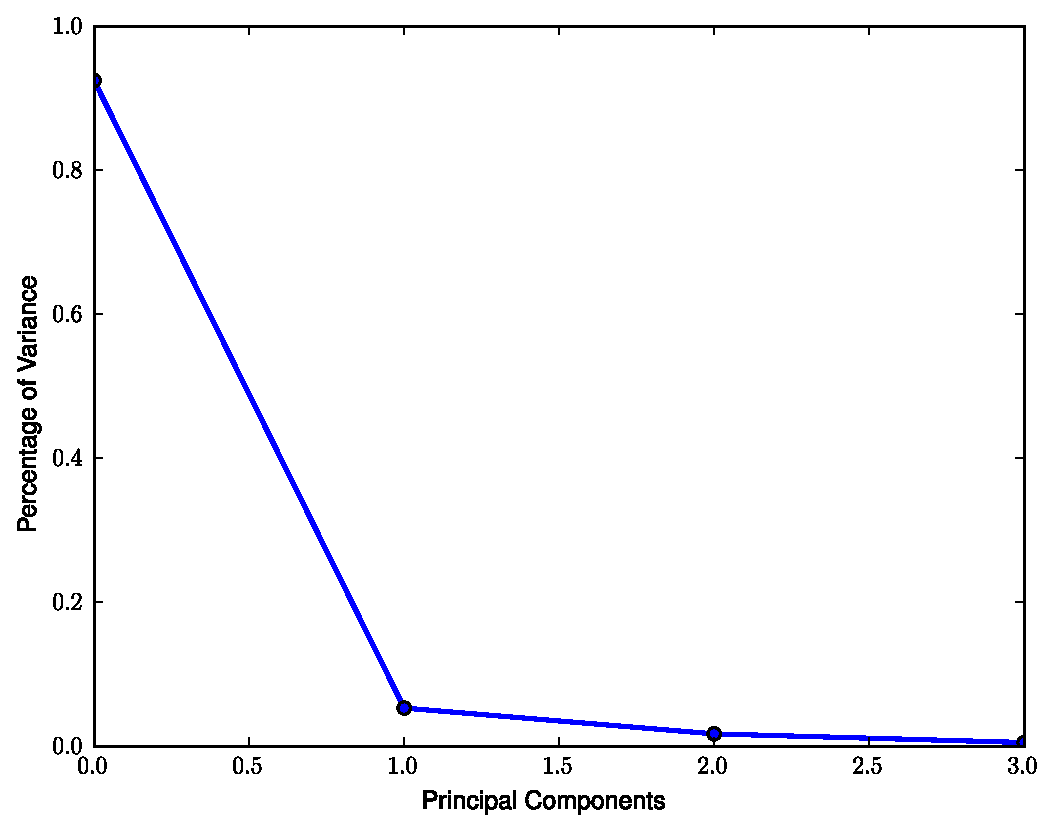
\includegraphics[width=\textwidth]{iris_scree.pdf}
\caption{Scree plot of the percentage of variance for PCA on the iris dataset.}
\label{fig:iris_scree}
\end{figure}
Upon examination, we see that there is a distinct change after the first principal component. This method is referred to as finding the "elbow" of the scree plot, in which case we consider all the principal components on the left of the elbow. In this case, that is simply the first principal component, which accounts for $92\%$ of the variance.
We can transform the observations from the original feature space by computing 
\begin{equation*}
\widehat{X} = U\Sigma
\end{equation*}
where $U$ and $\Sigma$ are from the truncated SVD found previously. We can then represent $\widehat{X}$ well by only keeping the first $K$ columns, where $K$ is the number of principal components retained. In this way, we have transformed our observations from the original feature space into an orthoganalized space, where the first several components explain most of the variance in the observations, allowing us to further reduce the dimensionality in a reasonable way.

In Figure \ref{fig:iris_pca} we display the transformed iris data set, plotting the first principal component against the second. We can see that this reduction helps us to see the distinctions between the three different species, using only two dimensions instead of the full four dimensions of the feature space.
\begin{figure}
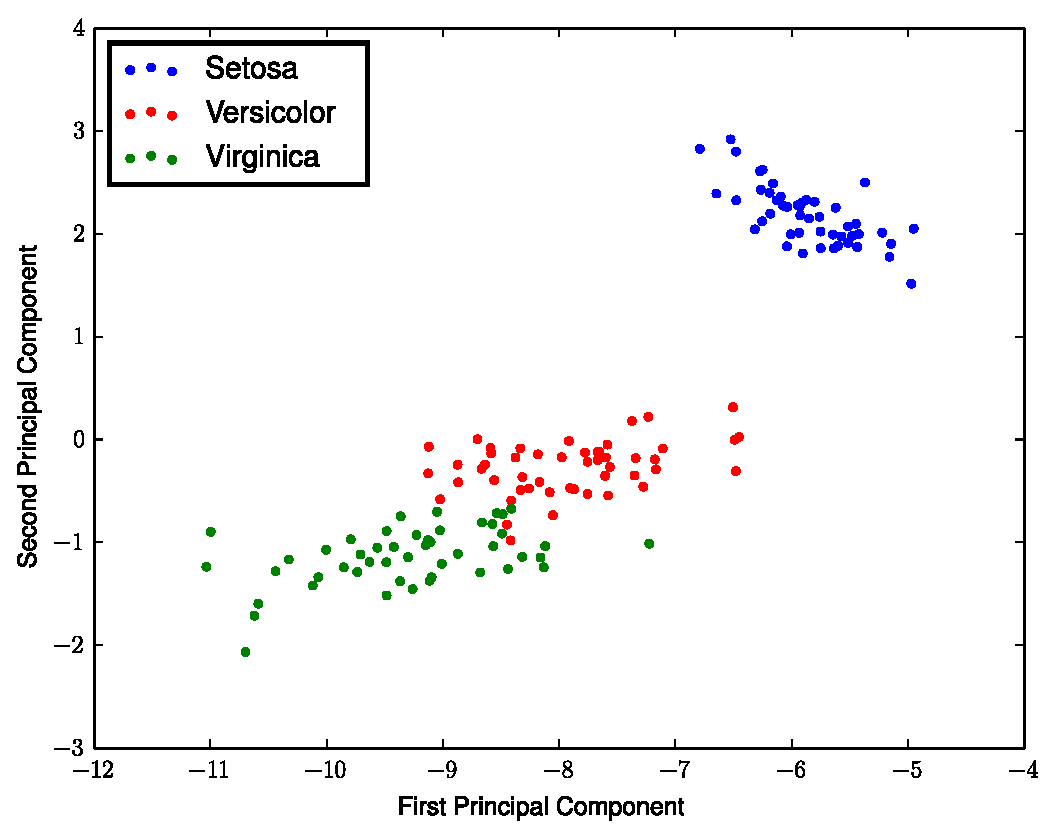
\includegraphics[width=\textwidth]{iris_pca.pdf}
\caption{Plot of transformed iris data, keeping only the first two principal components.}
\label{fig:iris_pca}
\end{figure}

To see this in a problem with more dimensions, suppose we have a large collection of documents. How can we find an article about PCA? We might consider simply choosing the article that contains the acronym \emph{PCA} the greatest number of times, but this is a crude method. A better way is to use a form of PCA itself on the collection of the documents. The idea is that we define the unique set of words occurring in the entire collection of documents as a vocabulary, and represent each document as a vector of count sums. Then PCA determines which words best distinguish between different documents.

In this case, the $i^{th}$ entry of a document's vector is $f_{i}$, where $f_{i}$ is defined to be the number of times term $i$ occurs in the document. We then represent the entire collection of documents as an $m \times n$ matrix $f$, where $m$ is the length of the vocabulary and $n$ is the number of documents in our collection, each column being a document vector. As expected, we let $f_{ij}$ be the number of times term $i$ occurs in document $j$.

We perform PCA on $f$ without centering the data so that we may retain the sparsity of $f$. We now have $f = T\Sigma D^{H}$. The $i^{th}$ row of $D$ is a vector corresponding to the $i^{th}$ document. We typically truncate these vectors, similar to identifying the important principal components of $t\!f$. We let $D_{i}$ denote the $i^{th}$ truncated row of $D$. Given a document $i$, we would like to find the document $j$ most similar to $i$, given that $i\neq j$. What we really need to compare are the vectors $D_{i}\Sigma$ and $D_{j}\Sigma$. Our metric of choice is the angle between two vectors, which is easily computable by considering the identity 
\begin{equation*}
\cos \theta_{ij} = \frac{D_{i}\Sigma \cdot D_{j}\Sigma}{\|D_{i}\Sigma\| \|D_{j}\Sigma\|}
\end{equation*}
where $\theta_{ij}$ is the angle between $D_{i}\Sigma$ and $D_{j}\Sigma$. If two document vectors have a small angle between them, then they are similar; a large angle signifies that they are quite different. Since $\cos \theta_{ij}$ is large whenever $\theta_{ij}$ is small, we seek to find 
\begin{equation*}
\argmax_{j} \frac{D_{i}\Sigma \cdot D_{j}\Sigma}{\|D_{i}\Sigma\| \|D_{j}\Sigma\|}
\end{equation*}
While this is the idea, in practice there are a few other steps we must take prior to the matrix decomposition. In any language, some words are so common that they provide no important information. We call these \emph{stop words}. Examples in English include \emph{the, a, an, and, I, we, you, it, there}, etc. Before processing any set of documents, we must remove all occurrences of stop words. We are going to consider the collection of all State of the Union addresses from 1945 to 2013, but these speeches are in an uncleaned format in the folder \emph{Addresses}, so we must first process them.

\begin{problem}
Using the function \li{loadStopwords} and the file 
\texttt{stopwords.txt} provided, read in the stop word list in Python. 
Use the functions \li{termlist}, \li{removeStopwords}, \li{uniq}, 
and \li{parseDocument} provided to create an array containing all of the unique 
terms encountered in the corpus that are not included in the stop word list. 
This is called the \emph{term list}.
\end{problem}

\begin{problem}
Write a function that accepts a file name, a list of stop words, and the term list 
found above, that will return a vector whose $i^{th}$ entry is the number of 
times the $i^{th}$ word from the term list occurs in the .txt file. 
Note that no word in the stop word list should ever contribute to any entry of this vector.
\end{problem}

\begin{problem}
Write a function that accepts a directory, a list of stop words, and the term list, 
that will make the term frequency matrix $t\!f$ as described above. 
Each column in $f$ should be the value returned by the function written in the 
previous problem for a particular file. In particular, $f$ should be a 
$m \times n$ matrix, where $m$ is the length of the term list and 
$n$ is the number of .txt files in the given directory.
\end{problem}

Not only is removing a predetermined set of stop words a good idea, 
but it's also important to consider that words appearing in few documents tend 
to provide more information than words occurring in every document. 
For example, while the word \emph{war} might not be considered a stop word, 
it is likely to appear in quite a few addresses, while \emph{Afghanistan} will not. 
Thus two speeches sharing the word \emph{Afghanistan} ought to be considered more 
related than two speeches sharing the word \emph{war}. 
So while $f_{ij}$ is a good measure of the importance of term $i$ in document $j$, 
we also need to consider some kind of global weight for each term $i$, 
indicating how important the term is over the entire collection. 
There are a number of different weights we could choose, but we choose to employ 
the following particular approach.

Let $t_{i}$ be the total number of times term $i$ appears in the entire 
collection of documents. 
Define 
\begin{equation*}
p_{ij} = \frac{f_{ij}}{t_{i}}
\end{equation*}
We then let 
\begin{equation*}
g_{i} = 1 + \sum_{j=1}^{n} \frac{p_{ij} \log (p_{ij} + 1)}{\log n}
\end{equation*}
where $n$ is the number of documents in the collection. 
We call $g_{i}$ the global weight of term $i$. 
We replace each term frequency in the matrix $f$ by weighting it globally. 
Specifically, we define 
\begin{equation*}
a_{ij} = g_{i} \log (f_{ij} + 1)
\end{equation*}
so we can consider these values to be a matrix $A$, which will take the place of 
$f$ as a matrix whose entries are both locally and globally weighted.

\begin{problem}
Write a function that accepts the term frequency matrix returned by your previous 
function, and which returns the matrix $A$ as described above. 
Perform PCA on $A$ as described above, remembering to \emph{not} center the data. 
Truncate the document vectors to retain the first $80\%$ of the variance in the data.
\end{problem}

\begin{problem}
Write a function that accepts the truncated document matrix, the list of file names 
for the documents, and an index $i$, and which returns the file name of the document 
most similar to the $i^{th}$ document. Find the speeches most similar to each of 
President George W. Bush's speeches, as well as the speeches most similar to 
each of President Obama's speeches.
\end{problem}
